\documentclass[11pt,twocolumn]{article}
\usepackage{lmodern,setspace,amsmath,amssymb,amsfonts,amsthm,graphicx,multicol,grffile,float}
\usepackage{authblk,url,csvsimple,cuted,dblfloatfix,stfloats,parskip}
\usepackage[a4paper, top=0.9in, bottom=1.05in, left=1.01in, right=1.01in]{geometry}
\usepackage[polish]{babel}
\usepackage[utf8]{inputenc}
\title{Optymalizacja kombinatoryczna - Sprawozdanie 1. \\ Algorytm zachłanny dla problemu job-shop}
\author{Dariusz Max Adamski 136674, Daniel Cieśliński 136695}
\affil{\{dariusz.adamski,daniel.cieslinski\}@student.put.poznan.pl}
\date{Data oddania:}

\begin{document}

\maketitle


\section*{Wstęp}

W tym sprawozdaniu przedstawiony będzie algorytm zachłanny, użyty do rozwiązania problemu szeregowania zadań (job-shop) \cite{ortools}.
Porównana będzie jakość rozwiązań w odniesieniu do ograniczenia dolnego instancji,
oraz czas wykonywania w zależności od wielkości instancji.


\section{Opis problemu}

Dla każdej instancji problemu szeregowania zadań,
zdefiniowane jest $\mathcal{J}$ zadań (jobs) oraz $\mathcal{M}$ maszyn.
Każde zadanie składa się z $\mathcal{M}$ operacji (tasks),
których kolejność jest znacząca.
$j$-ta operacja $i$-tego zadania musi być wykonywana na określonej maszynie $m_{ij}$,
przez określony czas $t_{ij}$.

Rozwiązanie uzyskujemy decydując o kolejnościach i
czasach startowych wykonywania operacji na każdej maszynie.

Makespan to czas w którym zostało zakończone ostatnie zadanie.
Celem programu jest minimalizacja tego kryterium.


\section{Opis rozwiązania}

\subsection{Algorytm zachłanny}

Zaimplementowany algorytm zachłanny działa na zasadzie symulacji,
to znaczy, że posiada zegar i w każdym takcie jeśli może przypisuje
wszystkie gotowe operacje do gotowych maszyn, 
w przeciwnym wypadku algorytm przechodzi do
czasu w którym można przypisać jakiejś maszynie jakąś operację,
lub jakaś operacja się zakończyła.

Program przechowuje i na bierząco aktualizuje informacje o tym
ile czasu dana maszyna będzie jeszcze zajęta (0 jeśli jest gotowa),
ile czasu pozostało do ukończenia aktualnej operacji w danym zadaniu,
ile pozostało operacji w danym zadaniu,
ile czasu pozostało do ukończenia zadania,
oraz ile zadań zakończyło się.

Decyzja o tym która operacja zostanie przypisana maszynie jest podejmowana za pomocą heurystyki SRTF
(shortest remaining time first). To znaczy, że jeżeli w danej chwili możemy do danej maszyny
przypisać jedną operację ze zbioru gotowych operacji, to wybierana jest operacja
która należy do zadania z najkrótszym czasem do ukończenia tego zadania.

Gdy wszystkie zadania zakończyły się, algorytm odczytuje aktualny czas,
czyli makespan. Następnie program zwraca rozwiązanie i kończy się sukcesem.


\section{Pomiary}

\subsection{Metodologia}

Instancje na których program był testowany to ,,tai'', ,,yn'', ,,fs'',
,,abz'', ,,ft'', ,,la'', ,,orb'', ,,swv'' i ,,dmu''.
Lącznie użyto 245 instancji problemu,
czyli wszystkich dostarczonych do zadania,
oraz instancje Demirkola \cite{bound}.

Program został przetestowany pod kątem poprawności,
na wszystkich instancjach,
przy użyciu sprawdzarki dostarczonej do zadania.

Dla algorytmu zachłannego czas wykonywania był mierzony 10 razy dla każdej instancji.
Czas wykonywania był mierzony nanosekundach na procesorze Intel i5-4670K.

\subsection{Czas wykonywania}

Zaimplementowany algorytm zachłanny działa bardzo szybko.
Czasy wykonywania wybranych instancji,
z tabeli w załączniku,
zawierają się w przedziale od 0.1 do 12 milisekund.
Najszybciej znajdywane jest rozwiązanie dla instancji ,,tai01'',
średnio zajmuje 0.249 milisekund.
Natomiast najwolniej znajdywane jest rozwiązanie dla instancji ,,tai74'',
średnio zajmuje 11.3 milisekund.

Dodatkowo dla instancji ,,tai25'' zostały zmierzone czasy wykonywania,
w zależności od ilości zadań branych pod uwagę.
Wyniki doświadczenia są przedstawione na rysunku \ref{tai_czas}.
Jak widać, czas wykonywania jest zależny od liczby zadań w instancji.

\begin{figure}[h!]
	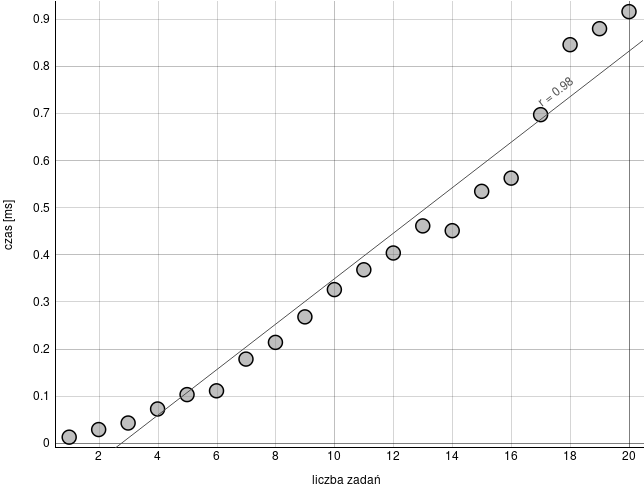
\includegraphics[width=\linewidth]{tai_czas.png}
	\caption{Czas wykonywania dla instancji tai25,
        w zależności od ilości zadań.
        Naniesiona linia trendu.
        \label{tai_czas}}
\end{figure}

\subsection{Porównanie jakości}

Aby ocenić jakość rozwiązań, w kolumnie ,,error'' tabeli \ref{tab1}
został obliczony błąd bezwględny w odniesieniu do ograniczenia dolnego,
według poniższego wzoru.
Alternatywnie można bezpośrednio porównać wartość ograniczenia dolnego/górnego
i makespan otrzymanego rozwiązania.

$$ error = \frac{|span - lb|}{lb} \cdot 100\% $$

Instancje zostały podzielone na pięć grup, w zależności od popełnionego błędu.
Wyniki są przedstawione na rysunku \ref{err_dist}.
Instancje ,,la'', ,,ft'' i ,,orb'' zostały pominięte z powodu braku informacji
o dolnym ograniczeniu rozwiązania.

\begin{figure}[h!]
	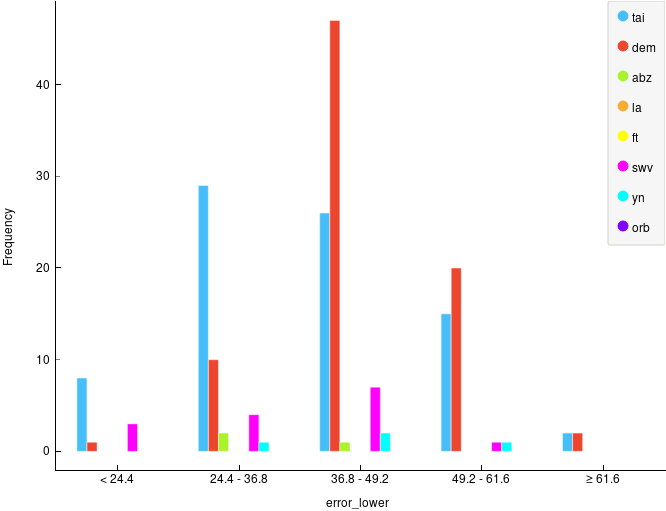
\includegraphics[width=\linewidth]{err_dist.png}
	\caption{Ilość instancji z błędem w danym przedziale, pogrupowane według źródła instancji \label{err_dist}}
\end{figure}

Algorytm zachłanny na większości instancji popełnia błąd z zakresu 37\% do 49\%.
Najwięcej instancji z przedziału 37\% do 49\% oraz 49\% do 60\% to instancje Demirkola \cite{dem}.
Najwięcej instancji z przedziału 0\% do 24\% oraz 24\% do 37\% to instancje Taillarda \cite{tai}.
Tylko pojedyńcze rozwiązania mają błąd większy niż 60\%.


\begin{table*}[b]
\centering
\begin{tabular}{l|rrrrrrrr}
    & $\mathcal{J}$ & $\mathcal{M}$ & lb  & ub   & span & error & $t_{avg}$ [ms] & $t_{stdev}$ [ms] \\ \hline
    tai20 & 20  & 15 & 1348 & 1348 & 2016 & 49\% & 8.7071e-1 & 1.8445e-1 \\
    tai21 & 20  & 20 & 1642 & 1642 & 2208 & 34\% & 8.3452e-1 & 7.9240e-2 \\
    tai22 & 20  & 20 & 1561 & 1600 & 2196 & 40\% & 9.5439e-1 & 1.2834e-1 \\
    tai23 & 20  & 20 & 1518 & 1557 & 2265 & 49\% & 9.0120e-1 & 1.1064e-1 \\
    tai24 & 20  & 20 & 1644 & 1644 & 2191 & 33\% & 1.0754e0 & 1.3551e-1 \\
    tai25 & 20  & 20 & 1558 & 1595 & 2161 & 38\% & 1.1765e0 & 9.5660e-2 \\ \hline
    tai01 & 15  & 15 & 1231 & 1231 & 1830 & 48\% & 2.49e-1 & 3.71e-3 \\
    tai74 & 100 & 20 & 5339 & 5339 & 6886 & 28\% & 1.13e1 & 1.38e0 \\
\end{tabular}
\caption{Parametry instancji, jakość rozwiązania i czasy wykonywania}
\label{tab1}
\end{table*}



\section{Wnioski}

Zaimplementowany algorytm zachłanny bardzo szybko znajduje rozwiązania,
jednak ich jakość nie jest zadowalająca.
Taki algorym może być stosowany w sytuacjach w których jest potrzeba
szybkiego wygenerowania rozwiązania,
na przykład w systemie operacyjnym.
Jednak gdy potrzebujemy bardziej optymalnego rozwiązania,
musimy zastosować inną metodę, lub zmienić heurystykę.


\newpage

\begin{thebibliography}{9}

\bibitem{ortools}
    \textit{The Job Shop Problem},
    \url{https://developers.google.com/optimization/scheduling/job_shop}

\bibitem{tai}
    \textit{Instancje Taillarda},
    \url{http://mistic.heig-vd.ch/taillard/problemes.dir/ordonnancement.dir/ordonnancement.html}

\bibitem{dem}
    \textit{Instancje Demirkola},
    \url{http://optimizizer.com/DMU.php}

\bibitem{bound}
    \textit{Ograniczenia dolne i górne instancji; Instancje Demirkola},
    \url{http://optimizizer.com/TA.php}

\end{thebibliography}

\end{document}

